\documentclass[12pt, a4paper]{article}

\usepackage[top=2cm, bottom=2cm, left=2cm, right=2cm]{geometry}

\usepackage{amssymb}
\usepackage{amsthm}
\usepackage{amscd}
\usepackage{amsmath}
\usepackage{enumitem}

\usepackage{multicol, fullpage}

\usepackage{esint} %Lines up double+ integrals
\usepackage[usenames,dvipsnames]{xcolor} % allows you to use color names, call this BEFORE you call TikZ
\usepackage{tikz, tikz-3dplot, pgfplots}
\usepackage{tkz-graph}
\usepackage{tensor}

%images
\usepackage{graphicx}
\usepackage{caption}
\usepackage{subcaption}

%\cancelto{thing cancelled to}{thing being cancelled}
\usepackage{cancel}

% compresses items in "itemize"
\setlist{nolistsep}

\usetikzlibrary{hobby}
\pgfplotsset{compat=1.8}


\usetikzlibrary{calc}


\setlength{\evensidemargin}{1in}
\addtolength{\evensidemargin}{-1in}
\setlength{\oddsidemargin}{1.5in}
\addtolength{\oddsidemargin}{-1.5in}
\setlength{\topmargin}{1in}
\addtolength{\topmargin}{-1.5in}

\setlength{\textwidth}{16cm}
\setlength{\textheight}{23cm}


\theoremstyle{plain}
\newtheorem{theorem}{Theorem}[section]
\newtheorem{lemma}{Lemma}
\newtheorem{proposition}{Proposition}
\newtheorem*{corollary}{Corollary}


\theoremstyle{definition}
\newtheorem{definition}{Definition}[section]
\newtheorem{notation}{Notation}
\newtheorem{question}{Question}
\newtheorem{conjecture}{Conjecture}[section]
\newtheorem{solution}{Solution}[section]
\newtheorem{example}{Example}[section]
\newtheorem{counter}{Counter Example}[section]


\theoremstyle{remark}
\newtheorem*{rem}{Remark}
\newtheorem*{note}{Note}


\def\proof{\noindent {\it Proof.} \hskip 0.1in}
\def\qed{\rightline{$\blacklozenge$}}

\newcommand{\RR}{\mathbb{R}}
\newcommand{\QQ}{\mathbb{Q}}
\newcommand{\NN}{\mathbb{N}}
\newcommand{\ZZ}{\mathbb{Z}}
\newcommand{\CC}{\mathbb{C}}
\newcommand{\II}{\mathbb{I}}

%
\begin{document}
%
%title and author details
\title{Cardiovascular Flow in Cylindrical Domain}
\author{Sean Kearns, Victor Ruiz\\
University of Colorado at Boulder\\
MATH5470}
\maketitle
\begin{abstract}
This project will briefly introduce the study of cardiovascular fluids, and discuss current analytical and numerical solutions. The Hagen-Poiseulle profile will be discussed as an example of the difficulties in constructing analytical solutions to hemodynamical problems. Also, the Arbitrary Lagrangian Eulerian numerical technique will be presented to demonstrate the value of numerical solutions to PDEs.
\end{abstract}
\section{Introduction}
Cardiovascular disease (CVD) claims over 17 million lives every year, and is currently the leading cause of death around the world. The difficulty with such an intricate collection of diseases is that detection is typically invasive and dangerous. Hence, having analytical or numerical blood flow models accurately describing the circulatory system would contribute to the creation of alternative methods of diagnosis, and treatment of CVDs $\cite{carotid}$.
%theoretical and historical construction (day 1), and physical/reality check (day 2)?

It was not until the 19th century that J.P. Poiseuille produced the first simplified mathematical model of fluid flow in a cylindrical pipe. Thereafter, contributors such as T. Young with the elasticity of arterial tissues and blood pressure propagation, O. Frank inventing the electric network analogy, and J. Womersley producing periodic pressure gradients have been associated with analytical hemodynamical problems $\cite{history}$. 

A modified version of the incompressible Navier-Stokes equations in cylindrical polar coordinates as demonstrated by Fung will be considered to expose the challenges associated with analytical solutions to blood flow problems $\cite{Biofluid}$. One particular numerical model using CT scans and axial geometry shown by Jane et. al. will also be considered to express the value of numerical solutions to cardiovascular fluid PDEs $\cite{carotid}$.


\newpage
\iffalse
\begin{figure}[ht!]
\centering
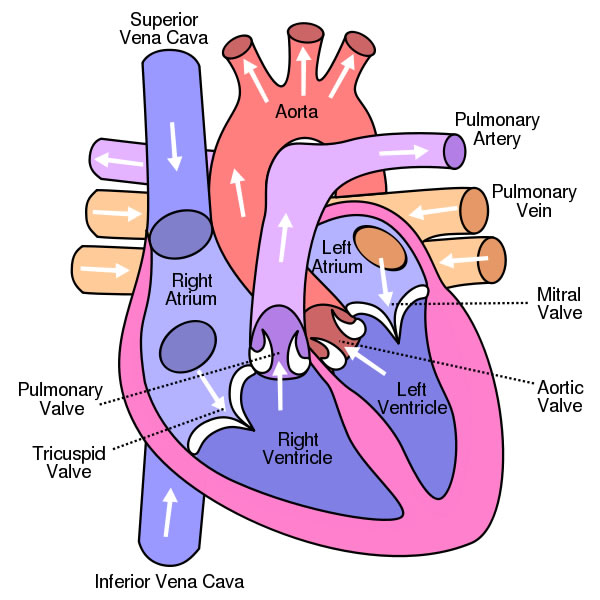
\includegraphics[width=150mm]{HeartDiagram.jpg}
\caption{Heart Diagram}
\end{figure}

\newpage
\fi
\section{Analytical Problem Formulation}

All variable assignments and assumptions will be considered here. Note that functions of time will not be observed.

\textbf{Variables}
\begin{align*}
u = u(y,z) &\equiv \; \text{Blood velocity} \\
p = p(y,z) &\equiv \; \text{Blood pressure} \\
\rho &\equiv \; \text{Blood density} \\
\mu &\equiv \; \text{Blood viscocity} \\
a &\equiv \; \text{radius} \\
r &\equiv \; \text{arbitrary radius such that} \; 0 \le r \le a
\end{align*}

$\vspace{.05in}$

\textbf{Assumptions}
\begin{itemize}
\item Incompressible flow: No divergence
\item Laminar flow: No turbulence 
\item Newtonian flow: Viscous stresses proportional to the rates of change of the fluid's velocity vector
\item No-slip condition: Fluid has zero velocity relative to a solid boundary (viscous fluid)
\item Horizontal tube: No gravity effecting the system
\item Symmetric flow: $u$ becomes a function of radius exclusively
\item Steady-state flow: Properties of the fluid do not change with time %(true since functions of time aren't considered)
\end{itemize}

$\vspace{.15in}$

Starting from the Navier-Stokes equations for blood flow in 3 dimensions
\begin{align}
\frac{\partial u}{\partial t} + u \frac{\partial u}{\partial x} + v \frac{\partial u}{\partial y} + w \frac{\partial u}{\partial z} = -\frac{1}{\rho} \frac{\partial p}{\partial x} + \frac{\mu}{\rho} \Delta u\\
\frac{\partial v}{\partial t} + u \frac{\partial v}{\partial x} + v \frac{\partial v}{\partial y} + w \frac{\partial v}{\partial z} = -\frac{1}{\rho} \frac{\partial p}{\partial y} + \frac{\mu}{\rho} \Delta v\\
\frac{\partial w}{\partial t} + u \frac{\partial w}{\partial x} + v \frac{\partial w}{\partial y} + w \frac{\partial w}{\partial z} = -\frac{1}{\rho} \frac{\partial p}{\partial z} + \frac{\mu}{\rho} \Delta w
\end{align}
over the circular cylindrical domain as expressed in the figure below from Y.C. Fung $\cite{Father}$,

\begin{figure}[ht!]
\centering
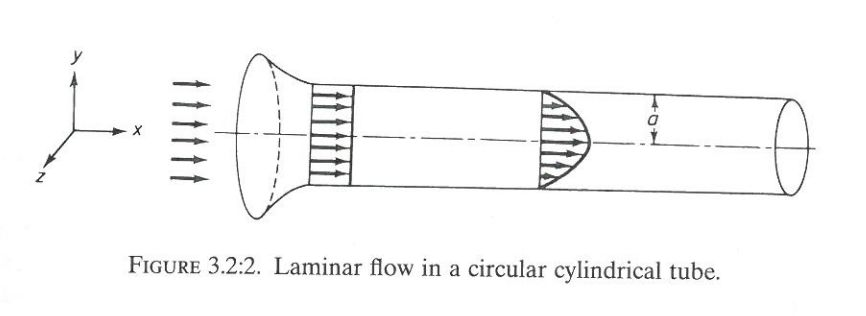
\includegraphics[width=100mm]{cardiovasculardomain.jpg}
\caption{Laminar flow in a circular cylindrical tube $\cite{Father}$.}
\end{figure}

\newpage

and assuming $v=w=0$ (velocity components in the $y$ and $z$ directions is zero) we have
\begin{align*}
\frac{\partial u}{\partial t} + u \frac{\partial u}{\partial x} + \cancelto{0}{v \frac{\partial u}{\partial y}} + \cancelto{0}{w \frac{\partial u}{\partial z}} = -\frac{1}{\rho} \frac{\partial p}{\partial x} + \frac{\mu}{\rho} \Delta u\\
\cancelto{0}{\frac{\partial v}{\partial t}} + u \cancelto{0}{\frac{\partial v}{\partial x}} + \cancelto{0}{v \frac{\partial v}{\partial y}} + \cancelto{0}{w \frac{\partial v}{\partial z}} = -\frac{1}{\rho} \frac{\partial p}{\partial y} + \frac{\mu}{\rho} \cancelto{0}{\Delta v}\\
\cancelto{0}{\frac{\partial w}{\partial t}} + u \cancelto{0}{\frac{\partial w}{\partial x}} + \cancelto{0}{v \frac{\partial w}{\partial y}} + \cancelto{0}{w \frac{\partial w}{\partial z}} = -\frac{1}{\rho} \frac{\partial p}{\partial z} + \frac{\mu}{\rho}  \cancelto{0}{\Delta w}
\end{align*}
and because $u$ is not a function of or the direction $x$, then we are left with
\begin{align}
\frac{1}{\rho} \frac{\partial p}{\partial x} &= \frac{\mu}{\rho} \Delta u \\
\frac{1}{\mu} \frac{\partial p}{\partial x} &=  \Delta u = \frac{\partial ^2 u}{\partial y^2} + \frac{\partial ^2 u}{\partial z^2}
\end{align}
Given a cylindrical domain, converting to cylindrical polar coordinates will simplify this problem considerably. From $x,y,z \rightarrow x,r,\theta$, suppose $r^2= y^2+z^2$, $y=r\cos\theta$, and $z=r\sin\theta$. Then
\begin{align*}
\frac{1}{\mu} \frac{\partial p}{\partial x} &= \frac{\partial ^2 u}{\partial y^2} + \frac{\partial ^2 u}{\partial z^2} \\
&=u_{rr}(r_y)^2+u_rr_{yy}+u_{\theta\theta}(\theta_y)^2 + u_\theta \theta_{yy} + u_{rr}(r_z)^2+u_rr_{zz}+u_{\theta\theta}(\theta_z)^2 + u_\theta \theta_{zz} \\
&=u_{rr}(\cos\theta)^2+u_r \left(\frac{\sin^2\theta}{r}\right)+u_{\theta\theta}\left(\frac{\sin^2\theta}{r^2}\right) + u_\theta \left( \frac{2\cos\theta\sin\theta}{r^2}  \right) \\
&+ u_{rr}(\sin\theta)^2+u_r \left(\frac{\cos^2\theta}{r}\right)+u_{\theta\theta}\left(\frac{\cos^2\theta}{r^2}\right) + u_\theta \left( \frac{-2\cos\theta\sin\theta}{r^2}  \right) \\
&= u_{rr} + \frac{1}{r} u_r + \frac{1}{r^2} u_{\theta\theta} \\
&= \frac{1}{r}\frac{\partial}{\partial r}\left( r\frac{\partial u}{\partial r} \right) + \frac{1}{r^2} \frac{\partial^2 u}{\partial \theta^2}
\end{align*} 
Assuming that the flow is symmetric, then $u=u(r)$, $\frac{\partial^2 u}{\partial \theta^2}=0$ and
\begin{align}
\frac{1}{r}\frac{\partial}{\partial r}\left( r\frac{\partial u}{\partial r} \right) = \frac{1}{\mu} \frac{\partial p}{\partial x}
\end{align}





\newpage
In order to solve for $u(r)$ and eventually the flow rate $Q$ we shall integrate equation $(6)$ twice with respect to $r$.

\begin{align*}
\frac{\partial}{\partial r} \left(  r \frac{\partial u}{\partial r} \right) &=  \frac{r}{\mu} \frac{\partial p}{\partial x} \\
\int \frac{\partial}{\partial r} \left(  r \frac{\partial u}{\partial r}   \right) \, dr &= \int \frac{r}{\mu} \frac{\partial p}{\partial x} \, dr \\
r \frac{\partial u}{\partial r}  &= \frac{r^2}{2\mu} \frac{\partial p}{\partial x} + A  \\
 \frac{\partial u}{\partial r}&= \frac{r}{2\mu} \frac{\partial p}{\partial x} + \frac{A}{r} \\
 \int \frac{\partial u}{\partial r} \, dr &= \int \frac{r}{2\mu} \frac{\partial p}{\partial x} + \frac{A}{r} \, dr \\
u&=\frac{r^2}{4\mu} \frac{\partial p}{\partial x} + A\ln{r} + B 
\end{align*}

The chosen boundary conditions must be applied before calculating the flow rate $Q$ through a slice of the cylinder.


With the assumptions that $\partial u/\partial r = 0$ at $r=0$ and $u=0$ at $r=a$, $A=0$ and $B= - \frac{a^2}{4\mu} \frac{\partial p }{\partial x}$.
 
$\vspace{.05in}$
To find $A$,
\begin{align*}
u  &= \frac{r^2}{4\mu} \frac{\partial p}{\partial x} + A\ln{r} + B  \\
0 = \partial u/\partial r &= \underbrace{\frac{r^2}{2\mu} \frac{\partial p}{\partial x}} + A \\
&\text{at $r=0$} \rightarrow A=0 
\end{align*}

To find $B$, 
\begin{align*}
0 = u  &= \frac{a^2}{4\mu} \frac{\partial p}{\partial x} + 0 \cdot \ln{r} + B  \\
B &=  - \frac{a^2}{4\mu} \frac{\partial p}{\partial x}
\end{align*}

After substituting $A$ and $B$, $u$ becomes
\begin{align}
u  &= \frac{r^2}{4\mu} \frac{\partial p}{\partial x} + A\ln{r} + B  \\
u  &= \frac{r^2}{4\mu} \frac{\partial p}{\partial x} - \frac{a^2}{4\mu} \frac{\partial p}{\partial x}  \\
u  &= - \frac{1}{4\mu} \frac{\partial p}{\partial x} \left[  a^2-r^2        \right]
\end{align}
Equation $(9)$ is the parabolic velocity profile of the $\it{Hagen}$-$\it{Poiseulle}$ $\it{flow}$, and is shown in figure 2. Integrating over the cross-sectional area of the cylinder provides the flow rate $Q$ as follows: 
\begin{align}
Q &= \int_0^{2\pi} \int_0^a - \frac{1}{4\mu} \frac{\partial p}{\partial x} \left[  a^2-r^2        \right] r \, drd\theta\\
    &= 2\pi \int_0^a - \frac{1}{4\mu} \frac{\partial p}{\partial x} \left[  a^2-r^2        \right] r \, dr\\
    &= 2\pi \left[ \frac{a^4}{16\mu}\frac{\partial p}{\partial x}-\frac{a^4}{8\mu}\frac{\partial p}{\partial x} \right]\\
    &=- \frac{\pi a^4}{8\mu} \frac{\partial p}{\partial x} 
\end{align}


\newpage

%%%%%%%%%%%%%%%%%%%%%%%%%%%%%%%%%%%%%%%%%%%%%%%%%%%%%
%%%%%%%%%%%%%%%%%%%%%%%%%%%%%%%%%%%%%%%%%%%%%%%%%%%%%



\section{Numerical Problem Formulation}

\begin{definition}[\bf{Runge-Kutta Method}]
A method for numerically integrating ordinary differential equations by using a trial step at the midpoint of an interval to cancel out the lower-order error terms.
\end{definition}

\textbf{Second-Order Formula}
\begin{align*}
{k}_{1} &= h\cdot f({x}_{n}, {y}_{n})\\
{k}_{2} &= h \cdot f \left( {x}_{n} + \frac{1}{2} h, {y}_{n} + \frac{1}{2} {k}_{1} \right)\\
{y}_{n+1} &= {y}_{n} + {k}_{2} + \mathcal{O} \left( {h}^{3} \right)\\
\end{align*}

\textbf{Fourth-Order Formula}
\begin{align*}
{k}_{1} &= h\cdot f({x}_{n}, {y}_{n})\\
{k}_{2} &= h \cdot f \left( {x}_{n} + \frac{1}{2} h, {y}_{n} + \frac{1}{2} {k}_{1} \right)\\
{k}_{3} &= h \cdot f \left( {x}_{n} + h, {y}_{n} + \frac{1}{2} {k}_{2} \right)\\
{k}_{4} &= h \cdot f \left( {x}_{n} + h, {y}_{n} + \frac{1}{2} {k}_{3} \right)\\
{y}_{n+1} &= {y}_{n} + \frac{1}{6}{k}_{1} + \frac{1}{3}{k}_{2}+ \frac{1}{3}{k}_{3}+ \frac{1}{6}{k}_{4} + \mathcal{O} \left( {h}^{5} \right)\\
\end{align*}
This method is reasonably simple and robust and is a good general candidate for numerical solution of differential equations when combined with an intelligent adaptive step-size routine. 

\noindent Let $\varphi$ be the map from the material domain to the spatial domain. 

\noindent let $\Phi$ be the map from the referential domain to the spatial domain. 

\noindent let $\Psi$ be the map from the referential domain to the material domain. 

\noindent let ${\Omega}_{M}$ denote the material domain and ${M}_{i}$ is a unit material. 

\noindent let ${\Omega}_{R}$ denote the referential domain. 

\noindent let ${\Omega}_{S}$ denote the spatial domain and ${S}_{i}$ is a unit of space. 

\newpage

\textbf{MAP OF DOMAINS} 

\noindent Thus,
\begin{flalign*}
\hspace{.75in} \varphi : {\Omega}_{M} \times [{t}_{0}, {t}_{\text{final}}) &\longrightarrow {\Omega}_{S} \times [{t}_{0}, {t}_{\text{final}})&\\
( \vec{M}, t) &\longmapsto \varphi( \vec{M}, t) = ( \vec{s}, t)&\\
& \longmapsto \Phi({\Psi}^{-1}( \vec{M}, t)) = ( \vec{s}, t) &
\end{flalign*}
which links $\vec{M}$ and $ \vec{S}$ in time by the law of motion, namely
\begin{align}
\vec{S} = \vec{S}(\vec{M}, t), t = t \hspace{1.1in}
\end{align}

\begin{enumerate}
\item The spatial coordinates $\vec{S}$ depend on both the material particle $\vec{M}$ and time $t$.

\item Physical time is measured by the same variable $v$ in both material and spatial domains. 
\end{enumerate}

\noindent Since $\varphi = \Phi \circ {\Psi}^{-1}$, let us define the mappings $\Phi$ (map from reference to spatial) and ${\Phi}^{-1}$ (map from material to referential).

\noindent Thus,
\begin{enumerate}
\item
\begin{flalign*}
\hspace{.4in} {\Phi}^{-1} : {\Omega}_{M} \times [{t}_{0}, {t}_{\text{final}} &\longrightarrow {\Omega}_{R} \times [{t}_{0}, {t}_{\text{final}})&\\
(\vec{M}, t) &\longmapsto \Phi(\vec{M}, t) = (\vec{R}, t)& \\
\end{flalign*}
\item
\begin{flalign*}
\hspace{.4in} {\Phi}^{-1} : {\Omega}_{R} \times [{t}_{0}, {t}_{\text{final}} &\longrightarrow {\Omega}_{S} \times [{t}_{0}, {t}_{\text{final}})&\\
(\vec{R}, t) &\longmapsto \Phi(\vec{R}, t) = (\vec{S}, t)&
\end{flalign*}
\end{enumerate}
$\Phi$ can be understood as the motion of the grid points in the spatial domain. 

${\Psi}^{-1}$ can be understood as the motion of the material form the perspective of the material. 


\begin{tikzpicture}
\begin{centering}
\draw plot [smooth cycle] coordinates {(5,0.25) (6,0.35) (6.5, 0.2) (7,0.5) (7,1.65) (6.5,2.75) (5.8,2.75) (5.3,1.45) (4.8,0.85) } node at (6.2,1.4) {$\Omega_S$};
\path[->] (3.1,1.7) edge [bend left] node[above] {$\varphi$} (5.0,1.7);
\draw plot [smooth cycle] coordinates {(1.0,.1)(1.5,.2)(2.8,.5)(2.9,1.5)(2.8,2.8)(1.4,2.5)(0.5,0.5)} node at (2.0,1.3) {$\Omega_M$};
\path[->] (1.6,0) edge [bend right] node[below] {$\varPsi$ \,\,} (2.7,-2.0);
\draw plot [smooth cycle] coordinates {(3.0,-2.1)(3.5,-2.2)(4.8,-2.0)(4.9,-3.3)(4.8,-4.0)(3.4,-4.0)(2.5,-2.5)} node at (3.9,-3.2) {$\Omega_R$};
\path[->] (4.9,-1.8) edge [bend right] node[below] {$\,\, \varPhi$} (5.75,0.0);
\end{centering}
\end{tikzpicture}
























\newpage


 \begin{thebibliography}{1}
 \bibitem{history} Alfio Quarteroni, {\em Modeling the Cardiovascular System--A Mathematical Adventure: Part I.} 2001: SIAM News 34.5 (2001): 1-3.

  \bibitem{n-seq} C Y Wang, {\em Exact solutions of the unsteady Navier-Stokes equations.} 1989: American Society of Mechanical Engineers.

  \bibitem{carotid}  Jhalique Jane R. Fojas, Rizalinda L. De Leon, {\em Carotid Artery Modeling Using the Navier-Stokes Equations for an Incompressible, Newtonian and Axisymmetric Flow.} 2013: Asia-Pacific Chemical, Biological $\&$ Environmental Engineering Society.

  \bibitem{Biofluid} Perumal Nithiarasu {\em Biofluid Dynamics.} 2008: Swansea University, United Kingdom.

  \bibitem{Father} Yuan-cheng Fung. {\em Biomechanics: circulation}. 1997: Springer.
APA	


  \end{thebibliography}

\end{document}